% presentation
\documentclass{beamer}

% \usetheme{Boadilla}
\usetheme{CambridgeUS}
\usecolortheme{dolphin}

% rus lang
\usepackage[main=russian,english]{babel}

% insert images
\usepackage{wrapfig}
\usepackage{graphicx}
\graphicspath{{./img/}, {../../plots/}}

% math
\usepackage{amsmath}
\usepackage{mathtools}
\usefonttheme[onlymath]{serif}
\newtheorem{rustheorem}{Теорема}

\newcommand{\at}[2][]{#1|_{#2}}
\newcommand{\eps}{\varepsilon}
\newcommand{\dd}[2]{\frac{\partial #1}{\partial #2}}

\DeclareMathOperator*{\argmin}{argmin}
\DeclareMathOperator{\sign}{sign}
\DeclareMathOperator{\K}{K}
\DeclareMathOperator{\R}{\mathbb{R}}
\DeclareMathOperator{\X}{\mathbb{X}}
\DeclareMathOperator{\Y}{\mathbb{Y}}
\DeclareMathOperator{\E}{\mathbb{E}}
\DeclareMathOperator{\V}{\mathbb{V}}

% algorithms
\usepackage[]{algorithm2e}

\title[Ансамбли]{Лекция 7. Композиции алгоритмов}
\subtitle{Основы интеллектуального анализа данных}
\author{Полузёров Т. Д.}
\institute{БГУ ФПМИ}
\date{}

\begin{document}
	
	\begin{frame}
		\titlepage
	\end{frame}
	
	
	\begin{center}
		\frametitle{Структура лекции}
		\tableofcontents
	\end{center}
	
	\section{Общие принципы}

	\subsection{Композиция}

	\begin{frame}
		\frametitle{Общие идеи}

		Имеется размеченная выборка $X^{\ell} = (x_i, y_i)_{i=1}^{\ell} \subset \X \times \Y$. 
		
		Задача --- приблизить истинную зависимость $y^{*}: \X \rightarrow \Y$

		\vspace{15pt}

		Ранее мы строили один сильный алгоритм $a(x) := C(b(x))$, такой что $\X \xrightarrow{b} \R \xrightarrow{C} \Y$.
		
		\vspace{15pt}

		Быть может лучше использовать несколько базовых алгоритмов $(b_i(x))_{i=1}^{k}$, а затем учесть ответы их всех
		$a(x) = C(F(b_1(x), \dots, b_k(x)))$. Тоесть $\X \xrightarrow{b} \alert{ \R^k \xrightarrow{F}} \R \xrightarrow{C} \Y$

		\vspace{15pt}

		Здесь $C$ --- решающее правило, $F$ --- агрегирующая операция.
	\end{frame}

	\begin{frame}
		\frametitle{}
		
		Для наших целей неважно как именно реализованы базовые алоритмы, они лишь должны поддерживать интерфейс
		\begin{itemize}
			\item $fit(X, Y)$ --- обучиться по выборке $X = (x, y)$
			\item $predict(X)$ --- выдать прогнозы $\hat{y} = b(X)$
		\end{itemize}

		\vspace{15pt}

		Мы же сфокусируемся на построении композиции и улучшении итогового качества.
		А именно: выбрать агрегирующую функцию и предложть метод обучения композиции.

		\vspace{15pt}

		Общие требования к $F$:
		\begin{itemize}
			\item $\min b_i \le F(b_1, \dots, b_k) \le \max b_i$
			\item $F(b_1(x), \dots, b_k(x))$ монотонно не убывает по всем $b_i$
		\end{itemize}	
	\end{frame}

	\subsection{Агрегирующая функция}

	\begin{frame}
		\frametitle{Примеры агрегирующих функций}
		\begin{itemize}
			\item простое голосование
			\[
			F(b_1, \dots, b_k) = \frac{1}{k} \sum_{i=1}^{k} b_i(x)
			\]
			\item взвешенное голосование, $\sum_{i=1}^{k} \alpha_i = 1, \hspace{5pt} \alpha_i \ge 0$
			\[
				F(b_1, \dots, b_k) = \sum_{i=1}^{k} \alpha_i b_i(x)
			\]
			\item смесь алгоритмов с функциями компетентности $g : \X \rightarrow \R$
			\[
				F(b_1, \dots, b_k) = \sum_{i=1}^{k} g_i(x) b_i(x)
			\]
		\end{itemize}
	\end{frame}

	\section{Беггинг}

	\subsection{Смещение и разброс}

	\begin{frame}
		\frametitle{Функионал риска}
		Рассмотрим задачу регрессии с квадратичной функцией потерь. Качество алгоритма $a$:
		\[
		Q(a) = \E_x \E_{X, \eps} [y(x, \eps) - a(x, X)]^{2}
		\]

		\begin{itemize}
			\item $X$ --- обучающая выборка
			\item $y = f(x) + \eps$ --- целевая зависимость, наблюдаемая с точностью до шума $\eps$
			\item $a(x, X)$ --- ответ алгоритма в точке $x$, обученного по выборке $X$
			\item $\E_x$ --- среднее по всем тестовым точкам, 
			\item $\E_{X, \eps}$ --- среднее по всем обучающим выборкам и случайному шуму
		\end{itemize}
	\end{frame}

	\begin{frame}
		\frametitle{Смещение и разброс}
		
		Ошибку можно предстваить в виде трех слагаемых:
		\[
		Q(a) = \E_x bias_X^2 (a) + 
		\E_x variance_X (a)
		+ \sigma^2
		\]
		где
		\begin{itemize}
			\item $bias_X(a) = f(x) - \E_x [a(x, X)]$ --- смещение
			\item $variance(a) = \E_X [ a(x, X) - \E_x[a(x, X)] ]^2$ --- разброс
			\item $\sigma^2 = \E_x \E_{\eps} [y(x, \eps) - f(x)]^2$ --- неустранимый шум
		\end{itemize}
	\end{frame}

	\begin{frame}
		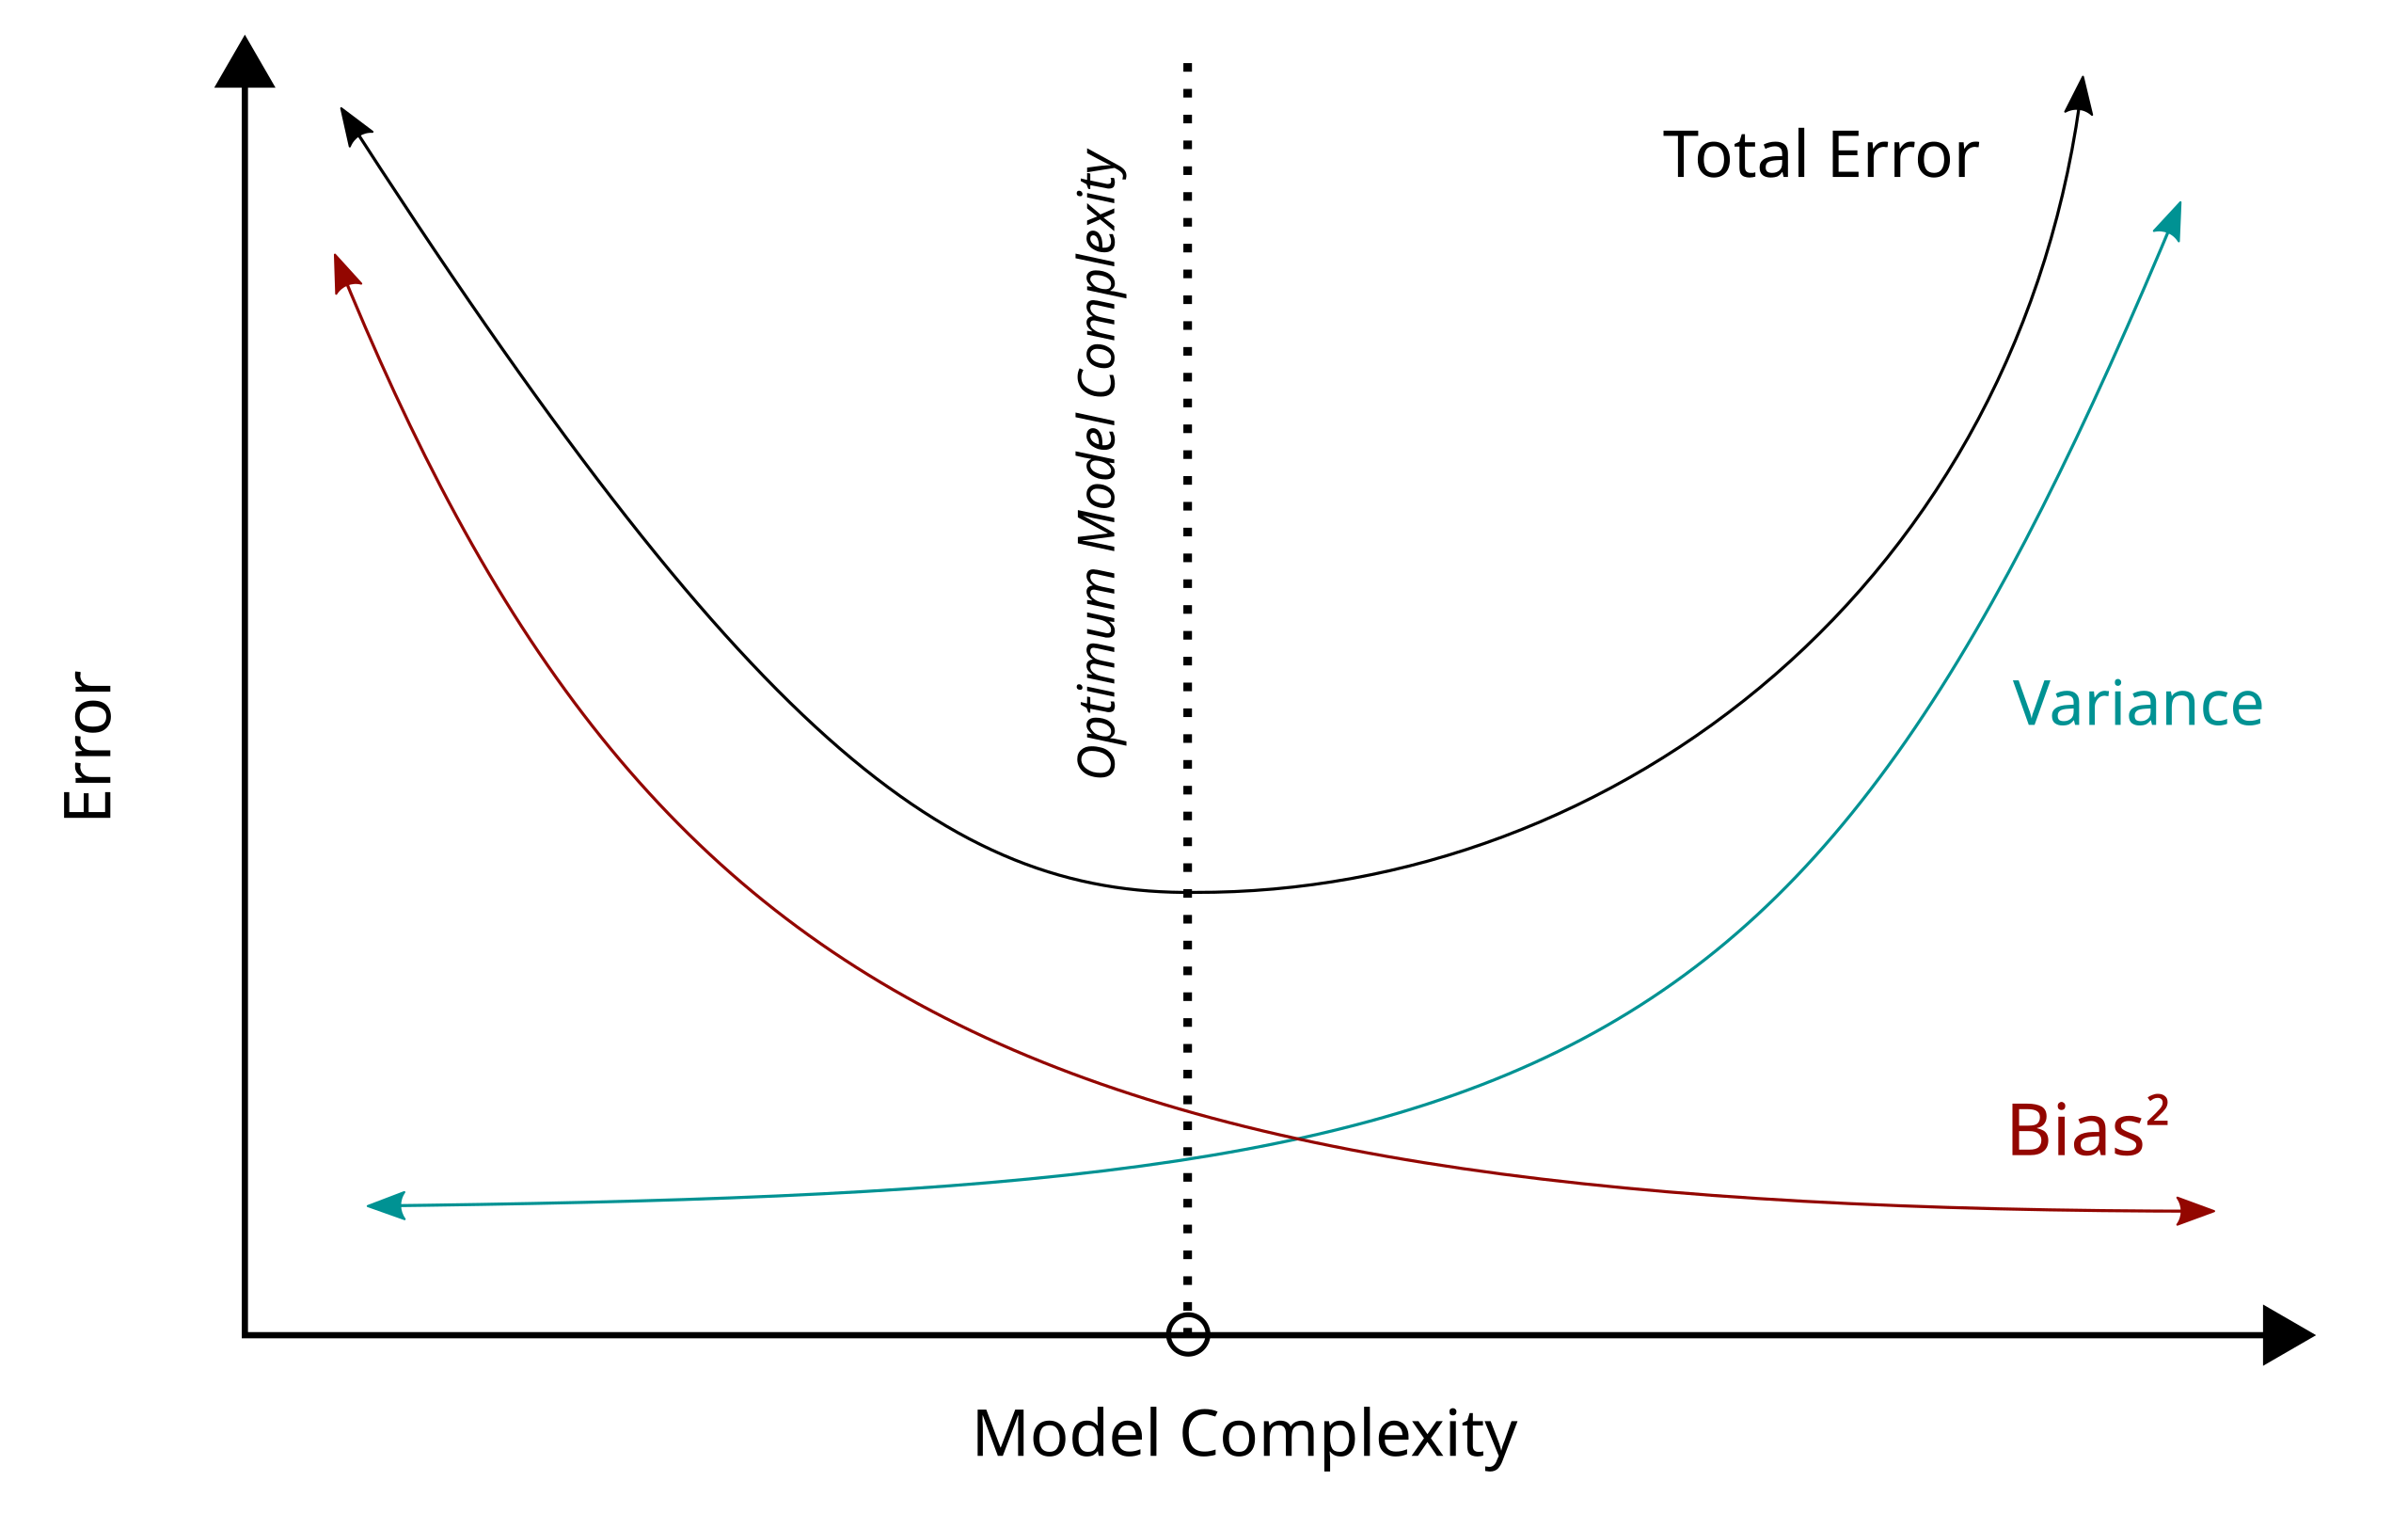
\includegraphics[width=1\textwidth]{img/bias_variance_tradeoff.png}	
	\end{frame}

	\begin{frame}
		\frametitle{Ошибка простого голосвания}

		Рассмотрим композицию --- простое голосование
		\[
		a(x) = \frac{1}{k} \left( b_1(x) + \dots + b_k(x) \right)
		\]

		\vspace{15pt}

		Как зависит смещние и разброс композиции от базового алгоритма $b$?
	\end{frame}

	\begin{frame}
		\frametitle{Смещение композиции}

		\begin{align*}
			bias_X(a) = 
			f(x) - \E_X[a(x, X)] = \\
			= f(x) - \E_X \left[\sum_{i=1}^{k} \frac{1}{k} b(x, X^i) \right] = \\
			= f(x) - \E_X b(x, X) = \\
			= bias_X(b)
		\end{align*}

		Смещение ансамбля определяется смещением базового алгоритма.
	\end{frame}

	\begin{frame}
		\frametitle{Разброс композиции}

		\begin{align*}
			variance_X(a) & = \E_X [ a(x, X) - \E_x[a(x, X)] ]^2 = \\
			& = \E_X \left[ \frac{1}{k} \sum_{i=1}^{k} b_i - \E_X \left[ \frac{1}{k} \sum_{i=1}^{k} b_i \right] \right]^2 = \\
			& = \frac{1}{k^2} \E_X \left[ \sum_{i=1}^{k} \left( b_i - \E_X b_i \right) \right]^2 = \\
			& = \frac{1}{k^2} \sum_{i=1}^{k} variance_X(b_i) + 
			\frac{1}{k^2} \sum_{i \ne j} cov(b_i, b_j)
		\end{align*}
	\end{frame}

	\subsection{Некоррелированность алгоритмов}

	\begin{frame}
		\frametitle{Некоррелированные базовые алгоритмы}

		В случае если базовые алгоритмы некоррелированны, то

		\begin{align*}
			variace_X(a) = \frac{1}{k^2} \sum_{i=1}^{k} variance_X(b_i) = \\ 
			= \frac{1}{k^2} \sum_{i=1}^{k} variance_X(b) = \\
			= \frac{1}{k} variance_X(b)
		\end{align*}

		Используя некоррелированную композицию алгоритмов, можно добиться уменьшения разброса 
		в $k$ раз!
	\end{frame}

	\begin{frame}
		\frametitle{Как добиться некоррелированности?}

		На практике строгое выполнение требования некоррелированности --- необязательно,
		достаточно, чтобы базовые алгоритмы были непохожи друг на друга.

		\vspace{15pt}

		Два способа увеличить непохожесть, строить $b_i(x)$:
		\begin{itemize}
			\item по случайной подвыборке объектов
			\item по псевдовыборке исходных объектов --- \textbf{бутстрап}
			\item по случайному подмножеству признаков --- \textbf{метод случайных подпространст}
		\end{itemize}
	\end{frame}

	\begin{frame}
		\frametitle{Бутстреп}

		Пусть имеется выборка $X$ объема $\ell$.

		\vspace{15pt}

		С помощью случайного \textbf{выбора с возвращением} сформируем новую <<выборку>> $X^1$ тоже объема $\ell$. 
		Полученную подвыборку называют \textbf{псевдовыборкой}.

		Проделаем эту операцию $k$ раз и получим $\{X^1, \dots, X^k\}$ псевдовыборок.

		\vspace{15pt}

		Такой метод получения псевдовыборок называется \textbf{бутстрепом} (bootstrap).

		\vspace{15pt}

		Применяется в статистике для проверки гипотез, построения доверительных интервалов \dots
	\end{frame}

	\subsection{Случайный лес}

	\begin{frame}
		\frametitle{Бэггинг}
		Беггинг (bootstrap aggregation) --- простое голосование, где при построении базовых алгоритмов используется
		бутстрап и метод случайных подпространств.

		\vspace{15pt}

		Можно внести модификации:
		\begin{itemize}
			\item ввести порог $\alpha$ и не добавлять $b_i$ если не достигает нужного качества
			\item обучение $b_i$ идет не по всей выборке $U_i \subset X^{\ell}$--- можно оценить качество на невиданных данных $X^{\ell} \setminus U_i$
		\end{itemize}
	\end{frame}

	\begin{frame}
		\frametitle{Общий алгоритм обучения бэггинга}

		\begin{algorithm}[H]
			\KwData{
				обучающая выборка $X^{\ell}$, 

				$k$ --- длина копозиции,

				$\alpha$ --- порог качества
				}
			\KwResult{базовые алгоритмы $b_1, \dots, b_k$}
			\For{$i = 1, \dots, k$}{
				$U_i := $ случайная подвыбрка размера $\ell^{'}$

				$G_i := $ случайное подмножество признаков размера $n^{'}$

				обучить $b_i$ по $G_i$ и $U_i$ 

				\If{$Q(b_i, U_i) < \alpha$}{
					добавить $b_i$ в композицию
				}

				оценить качество $Q(b_i, X^{\ell} \setminus U_i)$ на отложенных данных 
			}
		   \end{algorithm}
	\end{frame}

	\begin{frame}
		\frametitle{Случайный лес}
		Случайный лес (Random Forest) --- бэггинг над решающими деревьями.

		\vspace{15pt}

		Остаются вопросы
		\begin{itemize}
			\item Какой глубины $h$ строить деревья?
			\item Сколько признаков $n^{'}$ использовать для обучения?
			\item Сколько деревьев $k$ использовать в композиции?
		\end{itemize}
	\end{frame}

	\begin{frame}
		\frametitle{Глубина деревьев}

		Ошибка состоит из смещения и разброса.
		Разброс снижается за счет композиции, а смещение определяется смещением базового дерева.

		Поэтому необходимо использовать \textbf{деревья с низким смещением}.
		\begin{itemize}
			\item Неглубокие деревья имеют малое число параметров и поэтому строят только верхнеуровневые зависимости.
			При разных обучающих подвыборках алгоритмы не будут значительно отличатся (низкий разброс, высокое смещение).
			\item Глубокие деревья наоборот чересчур сильно подстраиваются под данные, поэтому имеют сильный разброс, но низкое смещение.
		\end{itemize}
		\vspace{15pt}

		Используем \textbf{глубокие деревья}.
	\end{frame}

	\begin{frame}
		\frametitle{Число признаков}

		Большое число признаков обеспечивает слабое различие деревьев, поэтому эффект
		от бэггинга --- слабый.

		С другой стороны, используя малое число признаков, базовые деревья будут слабыми.

		\vspace{15pt}

		Практическая рекомендация:
		\begin{itemize}
			\item Для задач регрессии --- $n^{'} = \lfloor n / 3 \rfloor$
			\item Для задач классификации --- $n^{'} = \lfloor \sqrt{n} \rfloor$
		\end{itemize}
	\end{frame}

	\begin{frame}
		\frametitle{Размер ансамбля}

		С ростом числа деревьев снижается разброс, но число признаков и вариантов подвыборок --- ограничены.
		Поэтому бесконечно уменьшать разброс не получится.

		\vspace{15pt}

		Имеет смысл построить график зависимости ошибки от числа деревьев и остановиться в тот момент, когда
		ошибка перестанет значимо уменьшатся

		\vspace{15pt}

		Так же ограничением может выступать время работы ансамбля. Большее число деревьев --- большее время принятия решения.

		Однако, алгоритмы стоятся независимо друг от друга и это позволяет распаралеливать построение отдельных деревьев.
	\end{frame}


	\begin{frame}
		\frametitle{Переход к взвешенному голосованию}

		Пусть уже построен набор базовых алгоритмов $b_1, \dots, b_k$.

		Взвешенная композиция
		\[
		a(x) = \sum_{i=1}^{k} \alpha_i b_i(x)
		\]
		есть ни что иное как линейная модель с новыми признаками --- ответами базовых моделей.

		\vspace{15pt}

		Настройка параметров
		\[
		Q(\alpha) = \sum_{i=1}^{\ell} \mathcal{L} (a(x_i, \alpha), y_i) \rightarrow \min_{\alpha}
		\]
	\end{frame}

	\section{Бустинг}

	\begin{frame}
		\frametitle{Идея бустинга}

		За основу возьмем взвешенное голосование
		\[
		a(x) = \sum_{i=1}^{k} \alpha_i b_i(x)
		\]
		Задан функционал качества
		\[
		Q(a) = \sum_{i=1}^{\ell} \mathcal{L} (a(x_i), y_i)
		\] 

		Основная идея --- строить последовательность $b_1, \cdots, b_k$ жадным способом.
		На итерации $t$ считаем вычисленными и зафиксированными $\alpha_1 b_1, \dots, \alpha_{t-1}b_{t-1}$.
	\end{frame}

	\subsection{Градиентный бустинг}
	
	\begin{frame}
		\frametitle{Градиентный бустинг}
		Рассмотрим наиболее общий алгоритм бустинга --- градиентный бустинг. 

		\vspace{15pt}

		Градиентный спуск для скалярной функции $Q(a) \rightarrow \min$ в пространстве ответов на обучающей выборке.

		Строится последовательность точек
		\[
		a_t = a_{t-1} - \alpha_t \dd{Q}{a} \at[\Big]{a = a_{t-1}}
		\]

		Схоже с добавлением нового базового алгоритма на каждой итерации.

		\vspace{15pt}
		
		Будем строить композицию, где $b_t$ приближает $\dd{Q}{a}$ в точке $a_{t-1}$

		\[
		b_t(x) \approx - \dd{Q}{a} \at[\Big]{a=a_{t-1}}
		\]
	\end{frame}
	
	\begin{frame}
		\frametitle{Приближение антиградиента}

		Приближение антиградиента можно сформулиоровать так

		\[
		g_{t-1, i} = \left( - \dd{Q}{a}\at[\Big]{a = a_{t-1}} \right)_i
		\]
		--- $i$-я компонента градиента, вычисленного в точке $a_{t-1}$ на всех объектах выборки
		\[
		b_t(x) = \arg \max_{b \in B} \sum_{i=1}^{\ell} \left( b(x_i) - g_{t-1, i} \right)^2
		\]

		Тоесть $b_t$ решает задачу регрессии, приближая антиградиент функции потерь.
	\end{frame}

	\begin{frame}
		\frametitle{Алгоритм градиентного бустинга}
		\begin{algorithm}[H]
			\KwData{
				обучающая выборка $X^{\ell}$, 
				}
			\KwResult{базовые алгоритмы и веса $\alpha_1 b_1, \dots, \alpha_k b_k$}
			Построить первый алгоритм $b_1(x)$

			\For{$t = 2, \dots, k$}{
				Вычислить
				
				$g := - \dd{Q}{a}\at{a=a_{t-1}}$
				
				Обучить алгоритм $b$: $x \rightarrow g$
				
				$b_t := \arg \min_{b} \sum_{j=1}^{\ell} \left( b(x_i) - g_i \right)^2$
				
				Подобрать $\alpha_t$ 
				
				$\alpha_t := \arg \min_{\alpha > 0} \sum_{j=1}^{\ell} L(a_{t-a} + \alpha b_t(x_j), y_j)$
			}
		   \end{algorithm}
	\end{frame}

	\begin{frame}
		\frametitle{Заключение}

		\begin{itemize}
			\item Композиции позволяют решать сложные задачи
			\item Почти всегда базовые алгоритмы --- решающие деревья
			\item Строить композиции целиком --- сложно. Поэтому базовые алгоритмы строятся по одному
			\item Построение беггинга можно распаралелить. Бустинга --- нет
			\item Обобщающая способность бустинга не ухудшается с ростом композиции
		\end{itemize}
	\end{frame}
\end{document}
